\chapter{Benchmarks}\label{chapter:benchmarks}
In this chapter the SIDH implementations introduced in \autoref{chapter:existing_sidh} are compared with each other. For this purpose, a benchmarking suite was developed, which allows the generation of comparable benchmarks between these implementations. To get a better understanding of the results, the chapter starts with \autoref{sec:benchmarks_methods} describing the tools and methodology used for benchmarking. The following implementations details of \autoref{sec:benchmarks_details} provide precise internals of the benchmarking suite. This might be used for further development of the software. A description of how to actually use the presented benchmarking suite will be given in \autoref{sec:benchmarks_usage}. Finally, the benchmarking results are listed in \autoref{sec:benchmarks_results}.

\section{Benchmarking Methodology}\label{sec:benchmarks_methods}
In order to generate independent and stable benchmarking results, the benchmarking suite runs within a virtual environment: \textit{Docker} is used to separate the running suite from the host operating system. This reduces the influence of resource intensive processes, which might falsify benchmarking results. Moreover, \textit{Docker} enables a portable and scalable software solution.
\\
In the following, the process of benchmarking is described within five steps. In a short version, the required steps are:

\begin{enumerate}
  \item Create the benchmarking source code
  \item Compile the benchmarking source code
  \item Run \textit{Callgrind}
  \item Run \textit{Massif}
  \item Collect benchmarks
\end{enumerate}

\subsubsection{Create the benchmarking code}
Each software libraries presented in \autoref{chapter:existing_sidh} implements various cryptographic primitives. To avoid overhead when calculating benchmarks, only the required functions to generate a SIDH key exchange should be called. Thus, a simple benchmarking file is provided for each implementation, which calls the appropriate underlying API. This benchmarking file must ensure that all required headers are imported, the API is called correctly and a \texttt{main}-function is provided.

\subsubsection{Compile the benchmarking code}
Once the benchmarking source code is created, it needs to be compiled to a binary. Therefore, all required dependencies (libraries, headers, sourc code, ..) need to be provided to the compiler. The benchmarking suite provides a \texttt{Makefile} for each implementation, where the compilation process is implemented.
All compilations performed for the benchmarking suit must use consistent compiler optimizations. This ensures the comparability of the outputs. Currently, the optimization flag \texttt{-O3} is passed to the gcc compiler. Note, that CIRCL is implemented in GO and therefore the go compiler is used for compilation. Since this compiler does not provide optimization flags, the default compiler optimizations are used \parencite{gowiki2020compiler}.
To be able to extract benchmarks for specific functions \textit{inlining} is disabled during compilation. The C programming language offers the following directive to disable \textit{inlining} for a function:
\begin{lstlisting}[language=C]
// This function will not be inlined by the compiler
void __attribute__ ((noinline)) no_inlining() {
// ...
}

// This function might be inlined by the compiler
void inlining() {
// ...
}
\end{lstlisting}
The go compiler can be directly invoked with a no-inlining (\texttt{-l}) flag:
\begin{lstlisting}[language=Go]
go build -gcflags "-l"
\end{lstlisting}

\subsubsection{Run \textit{Callgrind}}
\textit{Callgrind} records function calls of a binary. For each call the executed instructions are counted. Moreover, the tool provides detailed information about the callee and how often functions are called.Thus, the tool also provides information about execution hotspots of the binary. \textit{Callgrind} is part of \textit{Valgrind}, a profiling tool which allows deep analysis of executed binaries.\\
Callgrind is invoked on the command line via:
\begin{lstlisting}[language=Bash]
valgrind --tool=callgrind --callgrind-out-file=callgrind.out binary
\end{lstlisting}
The profiling data of callgrind is written to the file defined by \texttt{--callgrind-out-file}. This file might be analyzed using a graphical tool like \textit{KCachegrind} or any other analyzing script.
Running a binary using callgrind, slows down the execution times significantly. This is the main reason for the long execution times of the benchmarking suite. 

\subsubsection{Run \textit{Massif}}
\textit{Massif} measures memory usage of a binary, including heap and stack. \textit{Massif} is also part of the profiling tool \textit{Valgrind}. The tool creates multiple snapshots of the memory consumption during execution. Thus, one can extract the maximum memory consumption of a binary. The following command runs the \textit{Massif}:
\begin{lstlisting}[language=Bash]
valgrind --tool=massif --stacks=yes --massif-out-file=massif.out binary
\end{lstlisting}
The profiling data will be written to the file defined by \texttt{--massif-out-file}. \textit{Massif-visualizer} could be used to graphically analyze the data.

\subsubsection{Collect benchmarks}
Once the output files of \textit{Callgrind} and \textit{Massif} are produced, one can analyze the corresponding files to obtain:
\begin{enumerate}
\item Absolute instructions per function.
\item Maximum memory consumption during SIDH key exchange.
\end{enumerate}
This information is finally used by the benchmarking suite, to produce graphs and tables for further investigation. To receive reliable information, all benchmarks are executed multiple times.\\
To further increase the quality and reproducibility of the results, the cache of the virtual operating system is cleared, before \textit{Callgrind} and \textit{Massif} are executed. This is done via:
\begin{lstlisting}[language=Bash]
sync; sudo sh -c "echo 1 > /proc/sys/vm/drop_caches"
sync; sudo sh -c "echo 2 > /proc/sys/vm/drop_caches"
sync; sudo sh -c "echo 3 > /proc/sys/vm/drop_caches"
\end{lstlisting}


\section{Application Details}\label{sec:benchmarks_details}
The benchmarking suite is developed in Python3 on a Linux/Ubuntu operating system. Currently, the following implementations are included:
\label{sec:included_implementations}
\begin{itemize}
\item SIKE working on: \texttt{p434, p503, p610, p751}
	\begin{itemize}
	\item Sike reference implementation (\texttt{SIKE\_Reference})
	\item Sike generic optimized implementation (\texttt{SIKE\_Generic})
	\item Sike generic optimized and compressed implementation (\texttt{SIKE\_Generic\_Compressed})
	\item Sike x64 optimized implementation (\texttt{SIKE\_x64})
	\item Sike x64 optimized and compressed implementation (\texttt{SIKE\_x64\_Compressed})
	\end{itemize}
\item PQCrypto-SIDH working on: \texttt{p434, p503, p610, p751}
	\begin{itemize}
	\item PQCrypto-SIDH generic optimized implementation (\texttt{Microsoft\_Generic})
	\item PQCrypto-SIDH generic optimized and compressed implementation \\ (\texttt{Microsoft\_Generic\_Compressed})
	\item PQCrypto-SIDH x64 optimized implementation (\texttt{Microsoft\_x64})
	\item PQCrypto-SIDH x64 optimized and compressed implementation \\ (\texttt{Microsoft\_x64\_Compressed})
	\end{itemize}
\item CIRCL working on: \texttt{p434, p503, p610, p751}
	\begin{itemize}
	\item CIRCL x64 optimized implementation (\texttt{CIRCL\_x64})
	\end{itemize}
\end{itemize}
Furthermore, the benchmarking suite provides classical elliptic curve Diffie-Hellman (ECDH) based on OpenSSL. Since SIDH is a candidate to replace current Diffie-Hellman algorithms, ECDH is intended as reference value: The objective is it to compare optimized modern ECDH with quantum-secure SIDH.\\
Since each parameter set of SIDH meet a different security level (compare \autoref{sidh_security}) ECDH is also instantiated with different curves, each matching a SIDH security level. The used elliptic curves are namely:
\begin{enumerate}
\item \texttt{secp256r1} (openssl: \texttt{prime256v1} \parencite{turner2009elliptic}): 128 bit security matching \texttt{SIKEp434} \parencite{brown2010sec}
\item \texttt{secp384r1} (openssl: \texttt{secp384r1}): 192 bit security matching \texttt{SIKEp610} \parencite{brown2010sec}
\item \texttt{secp521r1} (openssl: \texttt{secp521r1}): 256 bit security  matching \texttt{SIKEp751} \parencite{brown2010sec}
\end{enumerate}
For each of these introduced implementations the application measures benchmarks. In the following sections detailed information about the internals of the suite is given. Beside the precise application flow (\autoref{sec:app_flow}), the internal class structure of the Python3 code is shown (\autoref{sec:app_structure}).

\subsection{Application Flow}\label{sec:app_flow}
This sections illustrates the application flow of the benchmarking suite (see \autoref{fig:app_flow}). Once triggered to run benchmarks, the following procedure is repeated for every implementation: The suite first compiles the benchmarking code. The binary is then executed multiple times to generate $N$ benchmarking results, respectively for \textit{Callgrind} and \textit{Massif}.
\\
Finally, the results are visualized in different formats. All resulting values are averages over N samples. Graphs compare the recorded instruction counts and the peak memory consumption among implementations instantiated with comparable security classes. The HTML and Latex tables lists all benchmarks per implementation and shows the standard derivation over $N$ samples.

\begin{figure}[H]
  \centering
  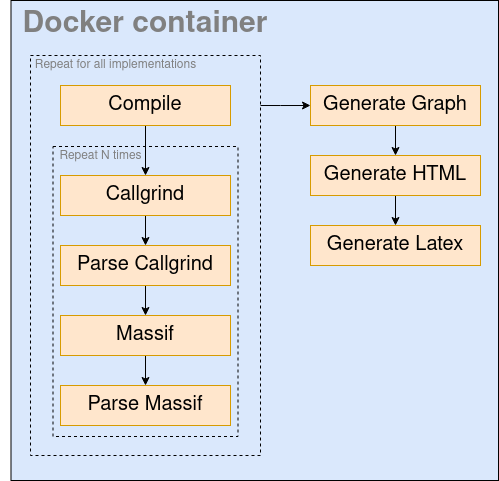
\includegraphics[width=0.8\textwidth]{benchmarks/application_flow}
  \caption[Flow chart of the benchmarking suite.]
  {Flow chart of the benchmarking suite. For each SIDH implementation, the source code is compiled and benchmarked multiple times. The benchmarking results are visualized in different format: Graphs, HTML and Latex.
  } \label{fig:app_flow}
\end{figure}




\subsection{Application Structure}\label{sec:app_structure}

This section covers the internal structure of the benchmarking suite. It illustrates, how each implementation is represented in code and how the benchmarking results are managed. To get a detailed description of the implemented functions have a look into the well-documented source code.

\subsubsection{Representation of concrete implementations}

The main logic of the benchmarking suite is placed within the class \texttt{BaseImplementation}. This class implements the logic of compiling code and measuring benchmarks. For each implementation which shall be benchmarked, a subclass of \texttt{BaseImplementation} is created (see \autoref{fig:uml}). These subclasses provide a link to the respective \textit{Makefile}, which is used by the \texttt{BaseImplementation} to compile code, run callgrind and run massif. Furthermore, each subclass can provide a set of arguments passed to the \textit{Makefile}.\\

\begin{figure}[H]
  \centering
  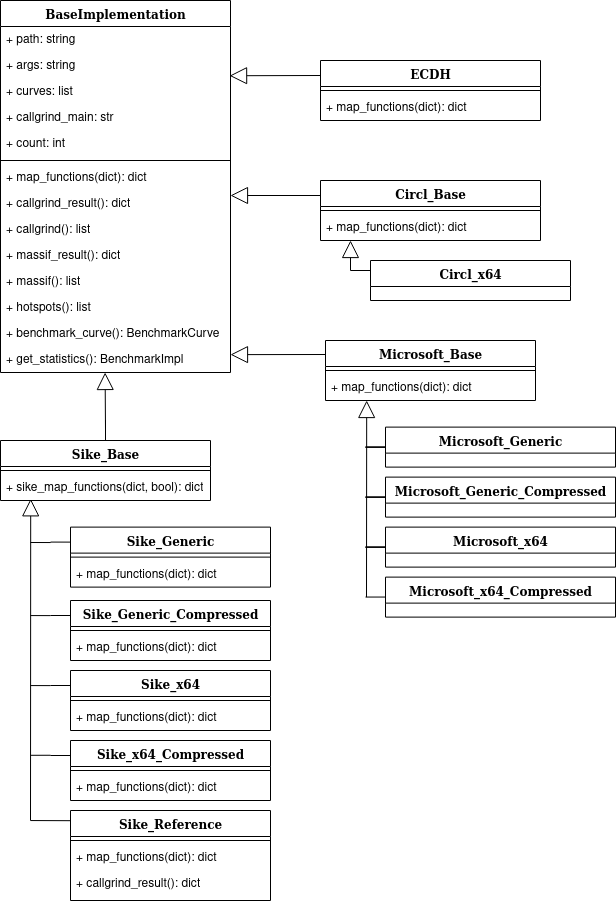
\includegraphics[width=0.8\textwidth]{benchmarks/uml}
  \caption[Class diagram for the all implementations supported by the benchmarking suite.]
  {Class diagram for the all implementations supported by the benchmarking suite. All concrete implementations of SIDH inherit from \texttt{BaseImplementation}. A \textit{Makefile} provided by each subclass specifies how the benchmarking code is built and run.} \label{fig:uml}
\end{figure}

\subsubsection{Representation of benchmarking results}
In order to ensure a clear analysis of the results the application implements a structure for the returned benchmarking values. Since each implementation can be run based on different parameter sets (in the terminology of the benchmarking suite this is called \textit{curves}) and for each curve different benchmarking values are processed, the following hierarchy is applied (see \autoref{fig:uml_results}).\\
The class \texttt{BechmarkImpl} represents the benchmarking results of a specific implementation. Therefore, the class manages a list of \texttt{BenchmarkCurve} objects, which contains benchmarks for a specific curve. Each benchmark for such a curve is represented by an instance of \texttt{Benchmark}. Thus, \texttt{BenchmarkCurve} holds a list of \texttt{Benchmark} objects.
\begin{figure}[H]
  \centering
  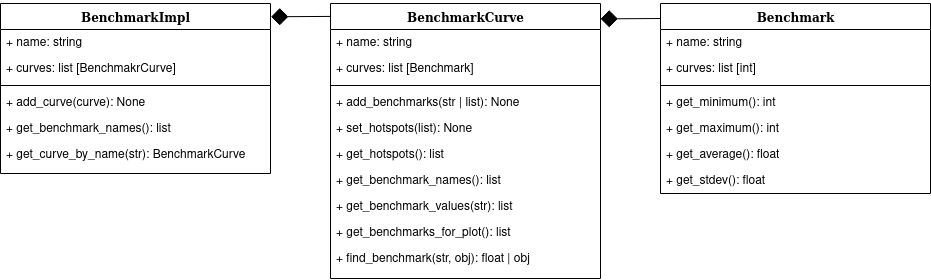
\includegraphics[width=1\textwidth]{benchmarks/uml_results}
  \caption[Class diagram for benchmarking results.]
  {Class diagram representing the management of the benchmarking results.}\label{fig:uml_results}
\end{figure}

\subsection{Adding Implementations}
To add a new implementation to the benchmarking suite it is helpful the have a look to existing implementations. Adding a SIDH implementation to the benchmarking suite requires the following steps:
\begin{enumerate}
\item Add a new folder into the \texttt{container/} folder of the root directory \\ \texttt{container/new\_implementation/}.
\item Create a file \texttt{container/new\_implementation/benchmark.c} that calls the SIDH key exchange API of the new implementation.
\item Add all necessary dependencies into \texttt{container/new\_implementation/} that are needed to compile \texttt{benchmark.c}. Note, maybe some changes in the \textit{Dockerfile} are necessary to install certain dependencies on the virtual operating system started by Docker.
\item Create a \texttt{Makefile}, that supports the following commands:
	\begin{itemize}
		\item build: Compile \texttt{benchmark.c} into the executable \\ \texttt{new\_implementation/build/benchmark}
		\item callgrind: Runs callgrind with the executable and stores the result in\\ \texttt{new\_implementation/benchmark/callgrind.out}.
		\item massif: Runs massif with the executable and stores the result in\\ \texttt{new\_implementation/benchmark/massif.out}.
	\end{itemize}
\item Add a new class to the source code, which inherits from \texttt{BaseImplementation}. You need to overwrite the \texttt{map\_functions()} method to map the specific API functions of the new implementation to the naming used within the benchmarking suite. The new class might look similar to this:

\begin{lstlisting}[language=Python]
class New_Implementation(BaseImplementation):
    def __init__(self, count):
        super().__init__(count=count,
				path=[path to Makefile], 
				args=[args for Makefile],
				callgrind_main=[name of main function],
				curves=curves)

    def map_functions(self, callgrind_result: dict) -> dict:
        res = {
            "PrivateKeyA": callgrind_result[[name of api function]],
            "PublicKeyA": callgrind_result[[name of api function]],
            "PrivateKeyB": callgrind_result[[name of api function]],
            "PublicKeyB": callgrind_result[[name of api function]],
            "SecretA": callgrind_result[[name of api function]],
            "SecretB": callgrind_result[[name of api function]],
        }
        return res
\end{lstlisting}
\item Import the created class into \texttt{container/benchmarking.py} and add the class to the \texttt{implementations} list:
\begin{lstlisting}[language=Python]
implementations =[
        #...
        New_Implementation,
    ]
\end{lstlisting}
\end{enumerate}
Once these steps are done the benchmarking suits is able to benchmark the new implementation.

\section{Usage}\label{sec:benchmarks_usage}
This section explains the usage of the benchmarking suite. Beside the execution of benchmarks, the application also provides unit tests for the implementation. Both tasks, running benchmarks and executing unit tests, need to run within the docker container. Thus, it is mandatory to \href{https://docs.docker.com/get-docker/}{install docker} on your system to run the benchmarking suite\footnote{Instructions for installing \textit{Docker}: https://docs.docker.com/get-docker/\\(The application was developed using Docker version 19.03.8, build \texttt{afacb8b7f0})}
To provide a easy to use interface for both tasks a script \textit{run.sh} is available. This script can be run with different arguments:
\begin{itemize}
\item Building the docker container:
\begin{lstlisting}[numbers=none,linewidth=4cm]
./run.sh build
\end{lstlisting}

\item Running unit tests within the docker container.
\begin{lstlisting}[numbers=none,linewidth=4cm]
./run.sh test
\end{lstlisting}
Testing the benchmarking suite runs for a while, since each implementation is compiled to verify the functionality of the \textit{Makefiles}. However, this procedure is logged while the unit tests are executed.

\item Running benchmarks within the docker container.
\begin{lstlisting}[numbers=none,linewidth=4cm]
./run.sh benchmark
\end{lstlisting}
This command triggers the \textit{benchmarking.py} script within the docker container. This script contains the entry logic of the benchmarking suite. It benchmarks all available implementations and generates different output formats (graphs, html, latex). It is configurable how often each benchmark should be measured: The variable \texttt{N} in \texttt{container/benchmarking.py} describes the amount of repetitions for \textit{callgrind} and \textit{massif}. Once the benchmarks are done, all output files can be inspected in the folder \texttt{data/} of your current directory. These files visualize average values over N samples. The output files are:
	\begin{itemize}
	\item \textit{XXX.png}: These files compare the absolute instruction count of all implementations, which were run on the XXX parameter set (XXX $\in {434, 503, 610, 751}$). Additionally, it contains a ECDH benchmark for comparison.
	\item \textit{XXX\_mem.png}: These files compare the peak memory consumption of all implementations, which were run on the XXX parameter set (XXX $\in {434, 503, 610, 751}$). Additionally, it contains a ECDH benchmark for comparison.

	\item \textit{cached.json}: This cache file contains all benchmarking results. It can be used as input for the benchmarking suite to use cached data instead of generating all benchmarks again. Since the benchmarking suite runs multiple hours if each implementation is evaluated N=100 times, this functionality provides great speed up if only the output data should change. To use the cached file as input, copy it to \texttt{container/.cached/cached.json} and run the benchmarking suite again.
	
	\item \textit{results.html}: This file lists detailed benchmarking results in a human readable HTML table. 
	
	\item \textit{results.tex}: This file contains the benchmarking results formatted in a latex table. The output is used for this document.
	\end{itemize}

\end{itemize}

\section{Results}\label{sec:benchmarks_results}
The results presented in this section were calculated on a x64 architecture (Intel(R) Core(TM) i5-6200U CPU @ 2.30GHz) running Ubuntu 20.04.1 LTS. The installed docker version was 19.03.8. 
The benchmarking suite was initialized to run \textit{callgrind} and \textit{massif} 100 times, respectively (e.g. $N$=100). This section visualizes the results of the benchmarking process. The docker container was invoked with the following command:
\begin{lstlisting}[numbers=none,linewidth=4cm]
./run.sh benchmark
\end{lstlisting}
The exact values measured (averages and standard derivation over $N$=100 samples) and the identified execution hotspots for each implementation described in \autoref{sec:included_implementations} can be found in addenda \ref{app:detailed_benchmarks}. This section visualizes all meaningful results. Note that this section does not interpret any results. A detailed analysis is given in \autoref{chapter:analysis}.
Each measured benchmark can be seen as a triplet chosen from:

\begin{center}
$[library]\:\:x\:\:[implementation]\:\:x\:\:[parameter\:set]$
\end{center}
Since this is hard to visualize in a single graph this section only shows the most important combinations. Possible choices are:

\subsubsection{Benchmarked libraries}
The benchmarked libraries are: \textit{SIKE}, \textit{PQCrypto-SIDH} (Microsoft) and \textit{CIRCL}.

\subsubsection{Implementations in each library}
When looking at the benchmarks of all libraries, one need to consider the characteristics of \textit{optimized} (generic and x64) implementations, \textit{compressed} implementations and \textit{reference} implementations. The \textit{reference} implementation by SIKE is by far the slowest version of the benchmarked SIDH key exchanges. \textit{Optimized} versions exploit hardware specific instructions leading to significantly reduced instruction counts. All \textit{compressed} versions benefit from smaller key sizes, however, they suffer from increased execution times and intense memory allocations. 
\subsubsection{Parameter sets for each implementation}
All libraries implement multiple parameter sets: \texttt{p434}, \texttt{p503}, \texttt{p610} or \texttt{p751}. Each implementation (\textit{compresed}, \textit{optimized} or \textit{reference}) might be initiated with one of these parameter sets. Each parameter set matches a NIST security level (see \autoref{sidh_security} for details).
\\\\
The first graph in \autoref{sec:results_all_curves} compares all possible SIDH security levels of the \texttt{SIKE\_x64} implementation. This demonstrates the performance differences of the implemented security classes. \\
A comparison among all implementations of SIKE is given in \autoref{sec:results_sike} - each initiated with \texttt{p434}. This quantifies the speed of compressed versions and the reference implementation compared to optimized versions.\\ 
Since the current SIDH libraries are also compared to the highly optimized ECDH openssl library, the figures in \autoref{sec:results_optimized} only consider the optimized implementations of all libraries. Additionally these graphs also list ECDH benchmarks. \\
Finally, \autoref{sec:results_compressed} compares all compressed implementations of the SIDH key exchange.\newpage

\subsection{SIDH security levels}\label{sec:results_all_curves}

\begin{figure}[H]
  \centering
  \includegraphics[width=0.9\textwidth]{benchmarks/all_curves/SIKE_x64}
  \caption[Overall instructions for all parameter sets via \texttt{SIKE\_x64}]
  {Overall instructions for \texttt{SIKE\_x64} initiated with all possible parameter sets.}
  \label{fig:results_ms_all_curves}
\end{figure}

\begin{figure}[H]
  \centering
  \includegraphics[width=0.9\textwidth]{benchmarks/all_curves/SIKE_x64_mem}
  \caption[Maximum memory consumption for all parameter sets via \texttt{SIKE\_x64}]
  {Maximum memory consumption in kilobytes of \texttt{SIKE\_x64} initiated with all possible parameter sets.}
  \label{fig:results_ms_all_curves_mem<}
\end{figure}

\subsection{SIKE Implementations}\label{sec:results_sike}
\begin{figure}[H]
  \centering
  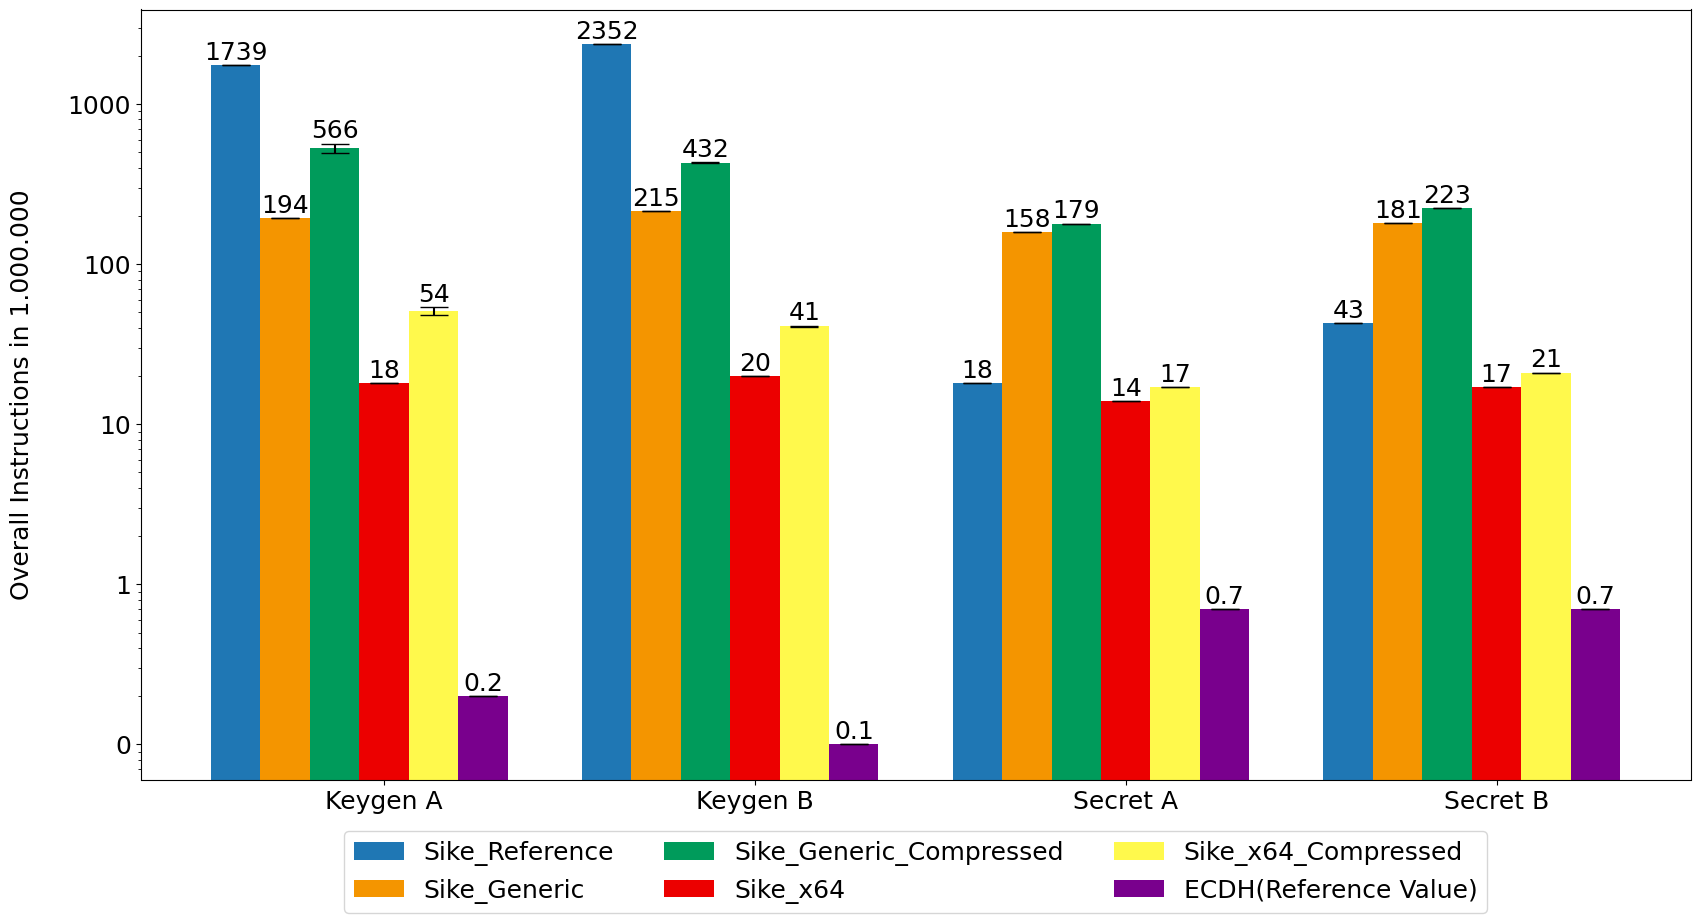
\includegraphics[width=0.9\textwidth]{benchmarks/sike/sike}
  \caption[Overall instructions SIKE]
  {Overall instructions for all SIKE implementations initialized with \texttt{p434}. The reference implementation is the slowest, the x64 optimized version is the fastest. These results meet intuitive expectations.}
  \label{fig:results_sike}
\end{figure}

\begin{figure}[H]
  \centering
  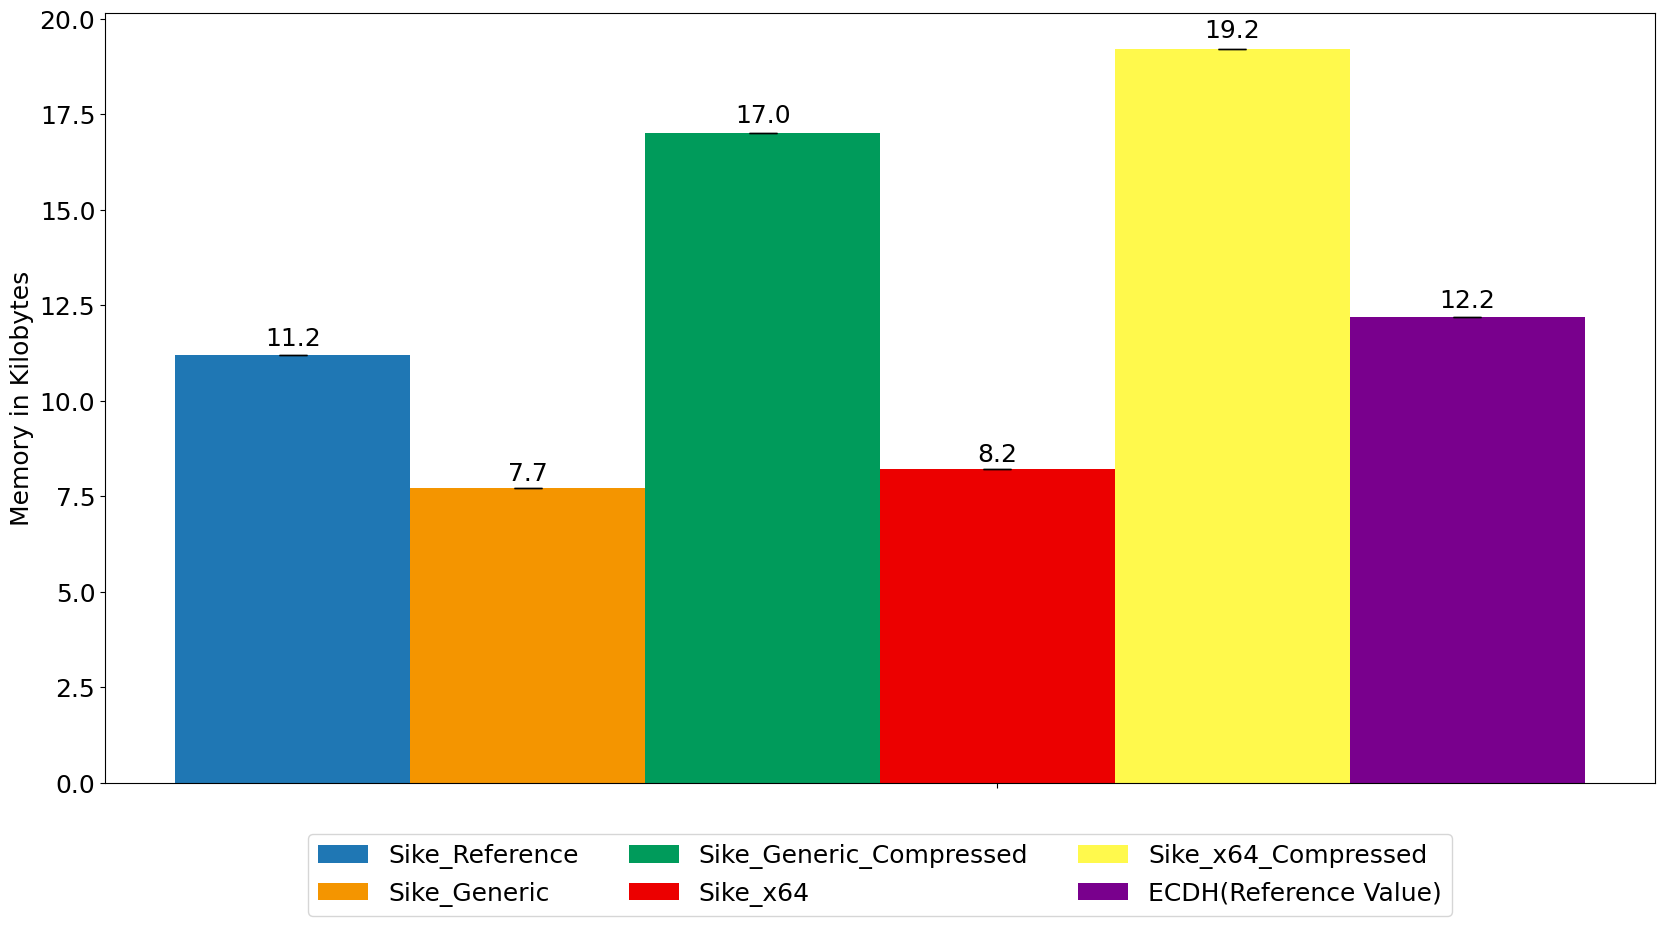
\includegraphics[width=0.9\textwidth]{benchmarks/sike/sike_mem}
  \caption[Maximum memory consumption SIKE]
  {Maximum memory consumption in kilobytes or all SIKE implementations initialized with \texttt{p434}. The required memory overhead of compressed versions is clearly visible.}
  \label{fig:results_sike_mem}
\end{figure}


\subsection{Optimized Implementations}\label{sec:results_optimized}
\subsubsection{Results matching NIST security level 1}
\begin{figure}[H]
  \centering
  \includegraphics[width=1\textwidth]{benchmarks/optimized/434}
  \caption[Overall instructions p434]
  {Overall instructions for SIDH parameter \texttt{p434} compared to ECDH via \texttt{secp256r1}.}
  \label{fig:results_opt_434}
\end{figure}

\begin{figure}[H]
  \centering
  \includegraphics[width=1\textwidth]{benchmarks/optimized/434_mem}
  \caption[Maximum memory consumption p434]
  {Maximum memory consumption in kilobytes for SIDH parameter \texttt{p434} compared to ECDH via \texttt{secp256r1}.}
  \label{fig:results_opt_434_mem}
\end{figure}

%\subsubsection{Results matching NIST security level 2}
%\begin{figure}[H]
%  \centering
%  \includegraphics[width=1\textwidth]{benchmarks/optimized//503}
%  \caption[Overall instructions p503]
%  {Overall instructions for SIDH parameter \texttt{p503} compared to ECDH via \texttt{secp384r1}.}
%  \label{fig:results_opt_503}
%\end{figure}
%
%\begin{figure}[H]
%  \centering
%  \includegraphics[width=1\textwidth]{benchmarks/optimized/503_mem}
%  \caption[Maximum memory consumption p503]
%  {Maximum memory consumption in kilobytes for SIDH parameter \texttt{p503} compared to ECDH via \texttt{secp384r1}.}
%  \label{fig:results_opt_503_mem}
%\end{figure}
%
%\subsubsection{Results matching NIST security level 3}
%\begin{figure}[H]
%  \centering
%  \includegraphics[width=1\textwidth]{benchmarks/optimized/610}
%  \caption[Overall instructions p610]
%  {Overall instructions for SIDH parameter \texttt{p610}.}
%  \label{fig:results_opt_610}
%\end{figure}
%
%\begin{figure}[H]
%  \centering
%  \includegraphics[width=1\textwidth]{benchmarks/optimized/610_mem}
%  \caption[Maximum memory consumption p610]
%  {Maximum memory consumption in kilobytes for SIDH parameter \texttt{p610}.}
%  \label{fig:results_opt_610_mem}
%\end{figure}

\subsubsection{Results matching NIST security level 5}
\begin{figure}[H]
  \centering
  \includegraphics[width=1\textwidth]{benchmarks/optimized/751}
  \caption[Overall instructions p751]
  {Overall instructions for SIDH parameter \texttt{p751} compared to ECDH via \texttt{secp521r1}.}
  \label{fig:results_opt_751}
\end{figure}

\begin{figure}[H]
  \centering
  \includegraphics[width=1\textwidth]{benchmarks/optimized/751_mem}
  \caption[Maximum memory consumption 751]
  {Maximum memory consumption in kilobytes for SIDH parameter \texttt{p751} compared to ECDH via \texttt{secp521r1}.}
  \label{fig:results_opt_751_mem}
\end{figure}

\subsection{Compressed implementations}\label{sec:results_compressed}

\subsubsection{Results matching NIST security level 1}
\begin{figure}[H]
  \centering
  \includegraphics[width=1\textwidth]{benchmarks/compressed/434}
  \caption[Overall instructions compressed p434]
  {Overall instructions for compressed SIDH parameter \texttt{p434}.}
  \label{fig:results_comp_434}
\end{figure}

\begin{figure}[H]
  \centering
  \includegraphics[width=1\textwidth]{benchmarks/compressed/434_mem}
  \caption[Maximum memory consumption compressed p434]
  {Maximum memory consumption in kilobytes for compressed SIDH parameter \texttt{p434}.}
  \label{fig:results_comp_434_mem}
\end{figure}

%\subsubsection{Results matching NIST security level 2}
%\begin{figure}[H]
%  \centering
%  \includegraphics[width=1\textwidth]{benchmarks/compressed//503}
%  \caption[Overall instructions compressed p503]
%  {Overall instructions for compressed SIDH parameter \texttt{p503}.}
%  \label{fig:results_comp_503}
%\end{figure}
%
%\begin{figure}[H]
%  \centering
%  \includegraphics[width=1\textwidth]{benchmarks/compressed/503_mem}
%  \caption[Maximum memory consumption compressed p503]
%  {Maximum memory consumption in kilobytes for compressed SIDH parameter \texttt{p503}.}
%  \label{fig:results_comp_503_mem}
%\end{figure}
%
%\subsubsection{Results matching NIST security level 3}
%\begin{figure}[H]
%  \centering
%  \includegraphics[width=1\textwidth]{benchmarks/compressed/610}
%  \caption[Overall instructions compressed p610]
%  {Overall instructions for compressed SIDH parameter \texttt{p610}.}
%  \label{fig:results_comp_610}
%\end{figure}
%
%\begin{figure}[H]
%  \centering
%  \includegraphics[width=1\textwidth]{benchmarks/compressed/610_mem}
%  \caption[Maximum memory consumption compressed p610]
%  {Maximum memory consumption in kilobytes for compressed SIDH parameter \texttt{p610}.}
%  \label{fig:results_comp_610_mem}
%\end{figure}

\subsubsection{Results matching NIST security level 5}
\begin{figure}[H]
  \centering
  \includegraphics[width=1\textwidth]{benchmarks/compressed/751}
  \caption[Overall instructions compressed p751]
  {Overall instructions for compressed SIDH parameter \texttt{p751}.}
  \label{fig:results_comp_751}
\end{figure}

\begin{figure}[H]
  \centering
  \includegraphics[width=1\textwidth]{benchmarks/compressed/751_mem}
  \caption[Maximum memory consumption compressed p751]
  {Maximum memory consumption in kilobytes for compressed SIDH parameter \texttt{p751}.}
  \label{fig:results_comp_751_mem}
\end{figure}

